\section{Introduzione}
Sempre più giochi da tavolo ormai vantano una versione digitale,
caratterizzata dalla possibilità di permettere agli utenti di giocare in
modalità multiplayer.
Allo stesso tempo sono ancora rare implementazioni completamente \emph{peer-to-peer} di
giochi multiplayer, spesso sono invece basate sull'architettura
\emph{client-server}. In questo documento descriveremo il nostro lavoro di
progettazione ed implementazione della versione digitale di un gioco da
tavolo con particolare interesse riguardo l'architettura di rete
distribuita utilizzata nella modalità multiplayer. \\

Carcassonne\footnote{\url{https://it.wikipedia.org/wiki/Carcassonne_(gioco)}} è un gioco da tavolo dei
primi anni 2000, che consiste nel creare un paesaggio medievale 
posizionando e accostando tra loro vari tipi di tessere, che rappresentano una parte di città, 
un tratto di strada, un campo coltivato o un monastero\footnote{Si fa riferimento
alla prima versione del gioco in cui non sono presenti fiumi, locande,
ponti o altri elementi di paesaggio introdotti dalle varie espansioni.}.
Completando più città, strade o monasteri attraverso tali tessere, i
giocatori (da 2 a 5 nella versione base del gioco) accumulano i punti necessari a vincere la partita.
Al fine di comprendere al meglio le prossime sezioni di questo documento, 
verranno illustrate ora le meccaniche del gioco.

\subsection{Carcassone}
All'inizio della partita, una specifica tessera è posizionata sul tavolo scoperta; 
le altre tessere vengono mescolate e posizionate coperte in un mazzo.
Ciascuna di tali tessere rappresenta un frammento di paesaggio, e può contenere uno o più dei seguenti elementi:

\begin{itemize}
	\item tratti di strada, inclusi incroci e curve;
    \item aree cittadine racchiuse da mura;
    \item campi che circondano le città e accolgono le strade;
    \item un monastero.
\end{itemize}


\begin{figure}[H]
\centering
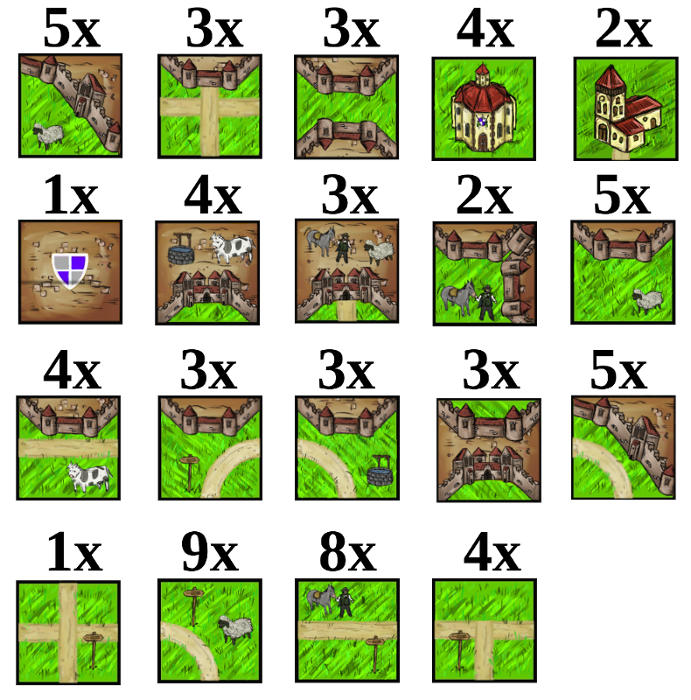
\includegraphics[width=\textwidth]{img/tiles.png}
\caption{Elenco delle tessere presenti nel gioco}
\label{img:tiles}
\end{figure}

A turno ogni giocatore estrae una tessera dal mazzo e la posiziona scoperta sul tavolo
a contatto con almeno una tessera già piazzata, in modo da mantenere la coerenza con le vicine, 
estendendo eventuali strade, campi, o citt\`a già presenti.

Dopo aver posizionato la tessera, il giocatore può decidere di piazzare
una pedina, detta \emph{seguace} o \emph{meeple}, su un elemento del paesaggio presente sulla tessera appena posizionata reclamandone la proprietà, a patto che non sia già posseduto da un altro giocatore.
Se un elemento diviene una congiunzione di due elementi dello stesso
tipo precedentemente non collegati, pu\`o ricadere sotto la propriet\`a di pi\`u giocatori; in questo caso, chi ha il numero maggiore di pedine sull'elemento rimane il proprietario, se sussiste un pareggio tutti i giocatori con il numero massimo di seguaci posizionati sull'elemento sono ritenuti proprietari e otterranno il punteggio relativo.

Quando un elemento viene completato, se ad esempio le mura di una città
vengono chiuse o se una strada ha due estremità, il proprietario acquisisce i relativi punti e tutte le pedine che erano sull'elemento vengono restituite ai relativi giocatori. Il punteggio di un
elemento è dipendente dal numero e dal tipo di tessere che lo compongono.

Unica eccezione viene fatta per i poderi, campi coltivati delimitati dagli altri elementi, che non vengono mai completati e sono soggetti ad un conteggio speciale al termine della partita.

Il gioco termina con il piazzamento dell'ultima tessera, dopo il quale viene effettuato il conteggio finale dei punteggi derivanti dagli elementi non completati posseduti dai giocatori; vince il giocatore che, dopo il conteggio finale, ha totalizzato più punti\footnote{Rimandiamo alla documentazione ufficiale di Carcassonne per ulteriori dettagli.}. \\

La semplice struttura del gioco e la sua organizzazione a turni rende
interessante l'approccio distribuito, in quanto si evita di incorrere in problemi 
di prestazioni tipici dei giochi reattivi. Questi ultimi infatti possono avere requisiti prestazionali molto stringenti. In
particolare spesso richiedono che le comunicazioni di rete siano a bassa
latenza al fine di evitare
artefatti grafici fastidiosi dovuti ai ritardi di rete o all'overhead di
comunicazione.\\
Come già accennato, il gioco da noi considerato necessita invece di
requisiti prestazionali più laschi, soprattuto per i lunghi tempi
decisionali degli utenti (comparati ai tempi di rete e computazionali).\\
